\chapter{\MinesweeperWinXPExampleChapterName}
\label{minesweeper_winxp}
\index{Windows!Windows XP}

\RU{Я не очень хорошо играю в Сапёра (Minesweeper), так что я попробую найти все скрытые мины в отладчике.}
\EN{I'm not very good at playing Minesweeper, so I'm going to reveal the hidden mines in the debugger.}

\index{\CStandardLibrary!rand()}
\index{Windows!PDB}
\RU{Как мы знаем, Сапёр располагает мины случайным образом, так что там должен быть генератор случайных чисел
или вызов стандартной функции Си \TT{rand()}.}
\EN{As we know, Minesweeper places mines randomly, so there has to be some kind of random number generator or
a call to the standard \TT{rand()} C-function.}
\RU{Вот что хорошо в реверсинге продуктов от Microsoft, так это то что часто есть \gls{PDB}-файл со всеми
символами (имена функций, \etc{}.).}
\EN{What is really cool about reversing Microsoft products is that there are \gls{PDB} 
file with symbols (function names, \etc{}).}
\RU{Когда я загружаю}\EN{When I load} \TT{winmine.exe} \RU{в}\EN{into} \IDA, \RU{она скачивает}\EN{it downloads the} 
\gls{PDB} \RU{файл именно для этого исполняемого файла и добавляет все имена}\EN{file exactly for this 
executable and shows all names}.

\RU{И вот оно, только один вызов}\EN{So here it is, the only call to} \TT{rand()} \RU{в этой 
функции}\EN{is this function}:

\begin{lstlisting}
.text:01003940 ; __stdcall Rnd(x)
.text:01003940 _Rnd@4          proc near               ; CODE XREF: StartGame()+53
.text:01003940                                         ; StartGame()+61
.text:01003940
.text:01003940 arg_0           = dword ptr  4
.text:01003940
.text:01003940                 call    ds:__imp__rand
.text:01003946                 cdq
.text:01003947                 idiv    [esp+arg_0]
.text:0100394B                 mov     eax, edx
.text:0100394D                 retn    4
.text:0100394D _Rnd@4          endp
\end{lstlisting}

\RU{Так её назвала \IDA и это было имя данное ей разработчиками Сапёра.}
\EN{\IDA named it so, and it was the name given to it by Minesweeper's developers.}

\RU{Ф-ция очень простая}\EN{The function is very simple}:

\begin{lstlisting}
int Rnd(int limit)
{
    return rand() % limit;
};
\end{lstlisting}

\RU{(В \gls{PDB}-файле не было имени ``limit''; это я назвал этот аргумент так.)}
\EN{(There was no ``limit'' name in the \gls{PDB} file; I named this argument.)}

\RU{Так что она возвращает случайное число в пределах от нуля до заданного предела}\EN{So it returns 
a random value from 0 to a specified limit}.

\TT{Rnd()} \RU{вызывается только из одного места, это функция с названием}\EN{is called only from one place, 
a function called} \TT{StartGame()}, 
\RU{и как видно, это именно тот код, что расставляет мины}\EN{and as it seems, this is exactly 
the code which place the mines}:

\begin{lstlisting}
.text:010036C7                 push    _xBoxMac
.text:010036CD                 call    _Rnd@4          ; Rnd(x)
.text:010036D2                 push    _yBoxMac
.text:010036D8                 mov     esi, eax
.text:010036DA                 inc     esi
.text:010036DB                 call    _Rnd@4          ; Rnd(x)
.text:010036E0                 inc     eax
.text:010036E1                 mov     ecx, eax
.text:010036E3                 shl     ecx, 5          ; ECX=ECX*32
.text:010036E6                 test    _rgBlk[ecx+esi], 80h
.text:010036EE                 jnz     short loc_10036C7
.text:010036F0                 shl     eax, 5          ; ECX=ECX*32
.text:010036F3                 lea     eax, _rgBlk[eax+esi]
.text:010036FA                 or      byte ptr [eax], 80h
.text:010036FD                 dec     _cBombStart
.text:01003703                 jnz     short loc_10036C7
\end{lstlisting}

\RU{Сапёр позволяет задать размеры доски, так что X (xBoxMac) и Y (yBoxMac) это глобальные переменные.}
\EN{Minesweeper allows you to set the board size, so the X (xBoxMac) and Y (yBoxMac) of the board are global variables.}
\RU{Они передаются в}\EN{They are passed to} \TT{Rnd()} \RU{и генерируются случайные координаты}\EN{and random 
coordinates are generated}.
\RU{Мина устанавливается инструкцией}\EN{A mine is placed by the} \TT{OR} \RU{на}\EN{instruction at} \TT{0x010036FA}. 
\RU{И если она уже была установлена до этого}\EN{And if it was placed before} 
(\RU{это возможно, если пара функций}\EN{it's possible if the pair of} \TT{Rnd()} 
\RU{сгенерирует пару, которая уже была сгенерирована}\EN{generates a coordinates pair which was already 
was generated}), 
\RU{тогда}\EN{then} \TT{TEST} \AndENRU \TT{JNZ} \RU{на}\EN{at} \TT{0x010036E6} 
\RU{перейдет на повторную генерацию пары}\EN{jumps to the generation routine again}.

\TT{cBombStart} \RU{это глобальная переменная, содержащая количество мин. Так что это цикл.}
\EN{is the global variable containing total number of mines. So this is loop.}

\RU{Ширина двухмерного массива это 32 (мы можем это вывести, глядя на инструкцию \TT{SHL}, которая умножает
одну из координат на 32)}\EN{The width of the array is 32 
(we can conclude this by looking at the \TT{SHL} instruction, which multiplies one of the coordinates by 32)}.

\RU{Размер глобального массива}\EN{The size of the} \TT{rgBlk} 
\RU{можно легко узнать по разнице между меткой}\EN{global array can be easily determined by the difference 
between the} \TT{rgBlk} 
\RU{в сегменте данных и следующей известной меткой}\EN{label in the data segment and the next known one}. 
\RU{Это}\EN{It is} 0x360 (864):

\begin{lstlisting}
.data:01005340 _rgBlk          db 360h dup(?)          ; DATA XREF: MainWndProc(x,x,x,x)+574
.data:01005340                                         ; DisplayBlk(x,x)+23
.data:010056A0 _Preferences    dd ?                    ; DATA XREF: FixMenus()+2
...
\end{lstlisting}

$864/32=27$.

\RU{Так что размер массива}\EN{So the array size is} $27*32$?
\RU{Это близко к тому что мы знаем: когда я попытался установить размер доски в установках Сапёра на}\EN{It is 
close to what we know: when I try to set board size to} $100*100$\RU{, то он установил размер}\EN{ in Minesweeper 
settings, it fallbacks to a board of size} $24*30$.
\RU{Так что это максимальный размер доски здесь}\EN{So this is the maximal board size here}.
\RU{И размер массива фиксирован для доски любого размера}\EN{And the array has a fixed size for any board size}.

\RU{Посмотрим на всё это в}\EN{So let's see all this in} \olly.
\RU{Я запустил Сапёр, присоединил (attach) \olly к нему и увидел содержимое памяти по адресу где массив}\EN{I ran 
Minesweeper, attaching \olly to it and I now see the memory dump at the address of the} 
\TT{rgBlk}\EN{ array}(\TT{0x01005340})
\footnote{\RU{Все адреса здесь для Сапёра под}\EN{All addresses here are for Minesweeper for} 
Windows XP SP3 English. 
\RU{Они могут отличаться для других сервис-паков}\EN{They may differ for other service packs}.}.

\RU{Так что у меня вышел такой дамп памяти массива}\EN{So I got this memory dump of the array}:

\lstinputlisting{examples/minesweeper/1.lst}

\olly, \RU{как и любой другой шестнадцатеричный редактор, показывает 16 байт на строку}\EN{like any other 
hexadecimal editor, shows 16 bytes per line}.
\RU{Так что каждая 32-байтная строка массива занимает ровно 2 строки}\EN{So each 32-byte array row occupies
exactly 2 lines here}.

\RU{Это уровень для начинающих (доска 9*9)}\EN{This is beginner level (9*9 board)}.

\RU{Тут еще какая-то квадратная структура, заметная визуально (байты 0x10)}\EN{There is some square 
structure can be seen visually (0x10 bytes)}.

\RU{Я нажал}\EN{I clicked} ``Run'' \InENRU \olly 
\RU{чтобы разморозить процесс Сапёра, потом нажал в случайное место окна Сапёра, попался на мине, но теперь
видны все мины}\EN{to unfreeze the Minesweeper process, then I clicked randomly at the Minesweeper window
and trapped into mine, but now I see all mines}:

\begin{figure}[H]
\centering
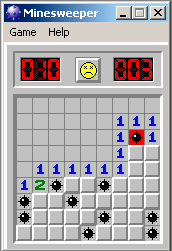
\includegraphics[scale=\FigScale]{examples/minesweeper/1.png}
\caption{\RU{Мины}\EN{Mines}}
\label{fig:minesweeper1}
\end{figure}

\RU{Сравнивая места с минами и дамп, мы можем обнаружить что 0x10 это граница, 0x0F\EMDASH{}пустой блок, 
0x8F\EMDASH{}мина.}
\EN{By comparing the mine places and the dump, we can conclude that 0x10 stands for border, 0x0F\EMDASH{}empty block, 0x8F---mine.}

\RU{Теперь я добавил комментариев и также включил все байты 0x8F в квадратные скобки:}
\EN{Now I added comments and also enclosed all 0x8F bytes into square brackets:}

\lstinputlisting{examples/minesweeper/2.lst}

\RU{Теперь я убрал все байты связанные с границами (0x10) и всё что за ними:}
\EN{Now I removed all \IT{border bytes} (0x10) and what's beyond those:}

\lstinputlisting{examples/minesweeper/3.lst}

\RU{Да, это всё мины, теперь это очень хорошо видно, в сравнении со скриншотом.}
\EN{Yes, these are mines, now it can be clearly seen and compared with the screenshot.}

\clearpage
\RU{Вот что интересно, это то что я могу модифицировать массив прямо в \olly.}
\EN{What is interesting is that I can modify the array right in \olly.}
\RU{Я убрал все мины заменив все байты 0x8F на 0x0F, и вот что у меня получилось в Сапёре}\EN{I removed 
all mines by changing all 0x8F bytes by 0x0F, and here is what I got in Minesweeper}:

\begin{figure}[H]
\centering
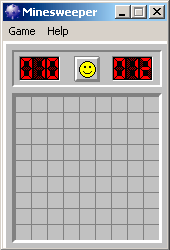
\includegraphics[scale=\FigScale]{examples/minesweeper/3.png}
\caption{\RU{Я убрал все мины в отладчике}\EN{I removed all mines in debugger}}
\label{fig:minesweeper3}
\end{figure}

\RU{Я также убрал их все и добавил их в первом ряду}\EN{I also moved all of them to the first line}: 

\begin{figure}[H]
\centering
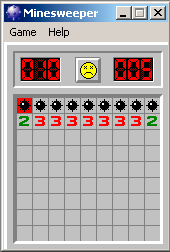
\includegraphics[scale=\FigScale]{examples/minesweeper/2.png}
\caption{\RU{Мины, установленные мною в отладчике}\EN{Mines I set in debugger}}
\label{fig:minesweeper2}
\end{figure}

\RU{Отладчик не очень удобен для подсматривания (а это была моя изначальная цель), так что я написал маленькую
утилиту для показа содержимого доски:}
\EN{Well, the debugger is not very convenient for eavesdropping (which was my goal anyway), so I wrote small utility
to dump the contents of the board:}

\lstinputlisting{examples/minesweeper/minesweeper_cheater.c}

\RU{Просто установите}\EN{Just set the} \ac{PID}
\footnote{PID \RU{можно увидеть в}\EN{it can be seen in} Task Manager 
(\RU{это можно включить в}\EN{enable it in} ``View $\rightarrow$ Select Columns'')} 
\RU{и адрес массива}\EN{and the address of the array} (\TT{0x01005340} \RU{для}\EN{for} Windows XP SP3 English) 
\RU{и она покажет его}\EN{and it will dump it}
\footnote{\RU{Скомпилированная версия здесь}\EN{The compiled executable is here}: 
\href{http://go.yurichev.com/17165}{beginners.re}}.

\RU{Она подключается к win32-процессу по \ac{PID}-у и просто читает из памяти процесса по этому адресу.}
\EN{It attaches itself to a win32 process by \ac{PID} and just reads process memory an the address.}

\section{\Exercises}

\begin{itemize}

\item \RU{Почему байты описывающие границы (0x10) присутствуют вообще?}
\EN{Why do the \IT{border bytes} (0x10) exist in the array?}
\RU{Зачем они нужны, если они вообще не видимы в интерфейсе Сапёра?}
\EN{What they are for if they are not visible in Minesweeper's interface?}
\RU{Как можно обойтись без них}\EN{How could it work without them}?

\item \RU{Как выясняется, здесь больше возможных значений (для открытых блоков, для тех на которых игрок установил
	флажок, \etc{}.).}
	\EN{As it turns out, there are more values possible (for open blocks, for flagged by user, \etc{}).}
\RU{Попробуйте найти значение каждого}\EN{Try to find the meaning of each one}.

\item \RU{Измените мою утилиту так, чтобы она в запущенном процессе Сапёра убирала все мины, 
или расставляла их в соответствии с каким-то заданным шаблоном.}
\EN{Modify my utility so it can remove all mines or set them in a fixed pattern that you want in the Minesweeper
process currently running.}

\item \RU{Измените мою утилиту так, чтобы она работала без задаваемого адреса массива и без \gls{PDB}-файла.}
\EN{Modify my utility so it can work without the array address specified and without a \gls{PDB} file.}
\RU{Да, вполне возможно автоматически найти информацию о доске в сегменте данных в запущенном процессе Сапёра.}
\EN{Yes, it's possible to find board information in the data segment of Minesweeper's running process automatically.}
\RU{Подсказка}\EN{Hint}: \myref{minesweeper_winxp_hint}.

\end{itemize}
